\subsection{Cơ cấu tổ chức nhóm/startup dự kiến}

Ở giai đoạn khởi đầu, nhóm lựa chọn vận hành theo \textbf{cơ cấu tổ chức theo
chức năng (functional structure)} kết hợp tinh thần làm việc phẳng (flat), trong
đó mỗi thành viên đảm nhận một mảng chức năng cốt lõi và cùng báo cáo trực tiếp
cho CEO/Project Lead. Đây là mô hình tổ chức phổ biến và phù hợp nhất với phần
lớn startup giai đoạn đầu, bởi nó xác định rõ vai trò, trách nhiệm gắn với mục
tiêu kinh doanh và tạo ra luồng báo cáo mạch lạc. Việc duy trì số tầng quản lý
tối thiểu giúp thông tin lưu thông nhanh, khuyến khích trao đổi cởi mở và rút
ngắn thời gian ra quyết định -- những yếu tố sống còn đối với một đội ngũ nhỏ,
nguồn lực hạn chế và cần kiểm chứng sản phẩm nhanh.


Trên cơ sở đó, nhóm vận hành như một doanh nghiệp thu nhỏ với năm vai trò chức
năng rõ ràng, đồng thời thiết lập kênh \textbf{thuê ngoài} cho các nghiệp vụ
chuyên sâu mà đội ngũ chưa có chuyên môn (kế toán, tư vấn pháp lý). Cách kết hợp
này tương ứng với mô hình mạng lưới (network model): tận dụng đối tác bên ngoài
để đội ngũ nội bộ tập trung vào năng lực cốt lõi là phát triển sản phẩm và tiếp
cận khách hàng, đồng thời tiết kiệm chi phí cố định trong giai đoạn đầu. Cơ cấu
tổ chức dự kiến được trình bày trong Hình~\ref{fig:cocau-to-chuc}.

\begin{figure}[H]
    \centering
    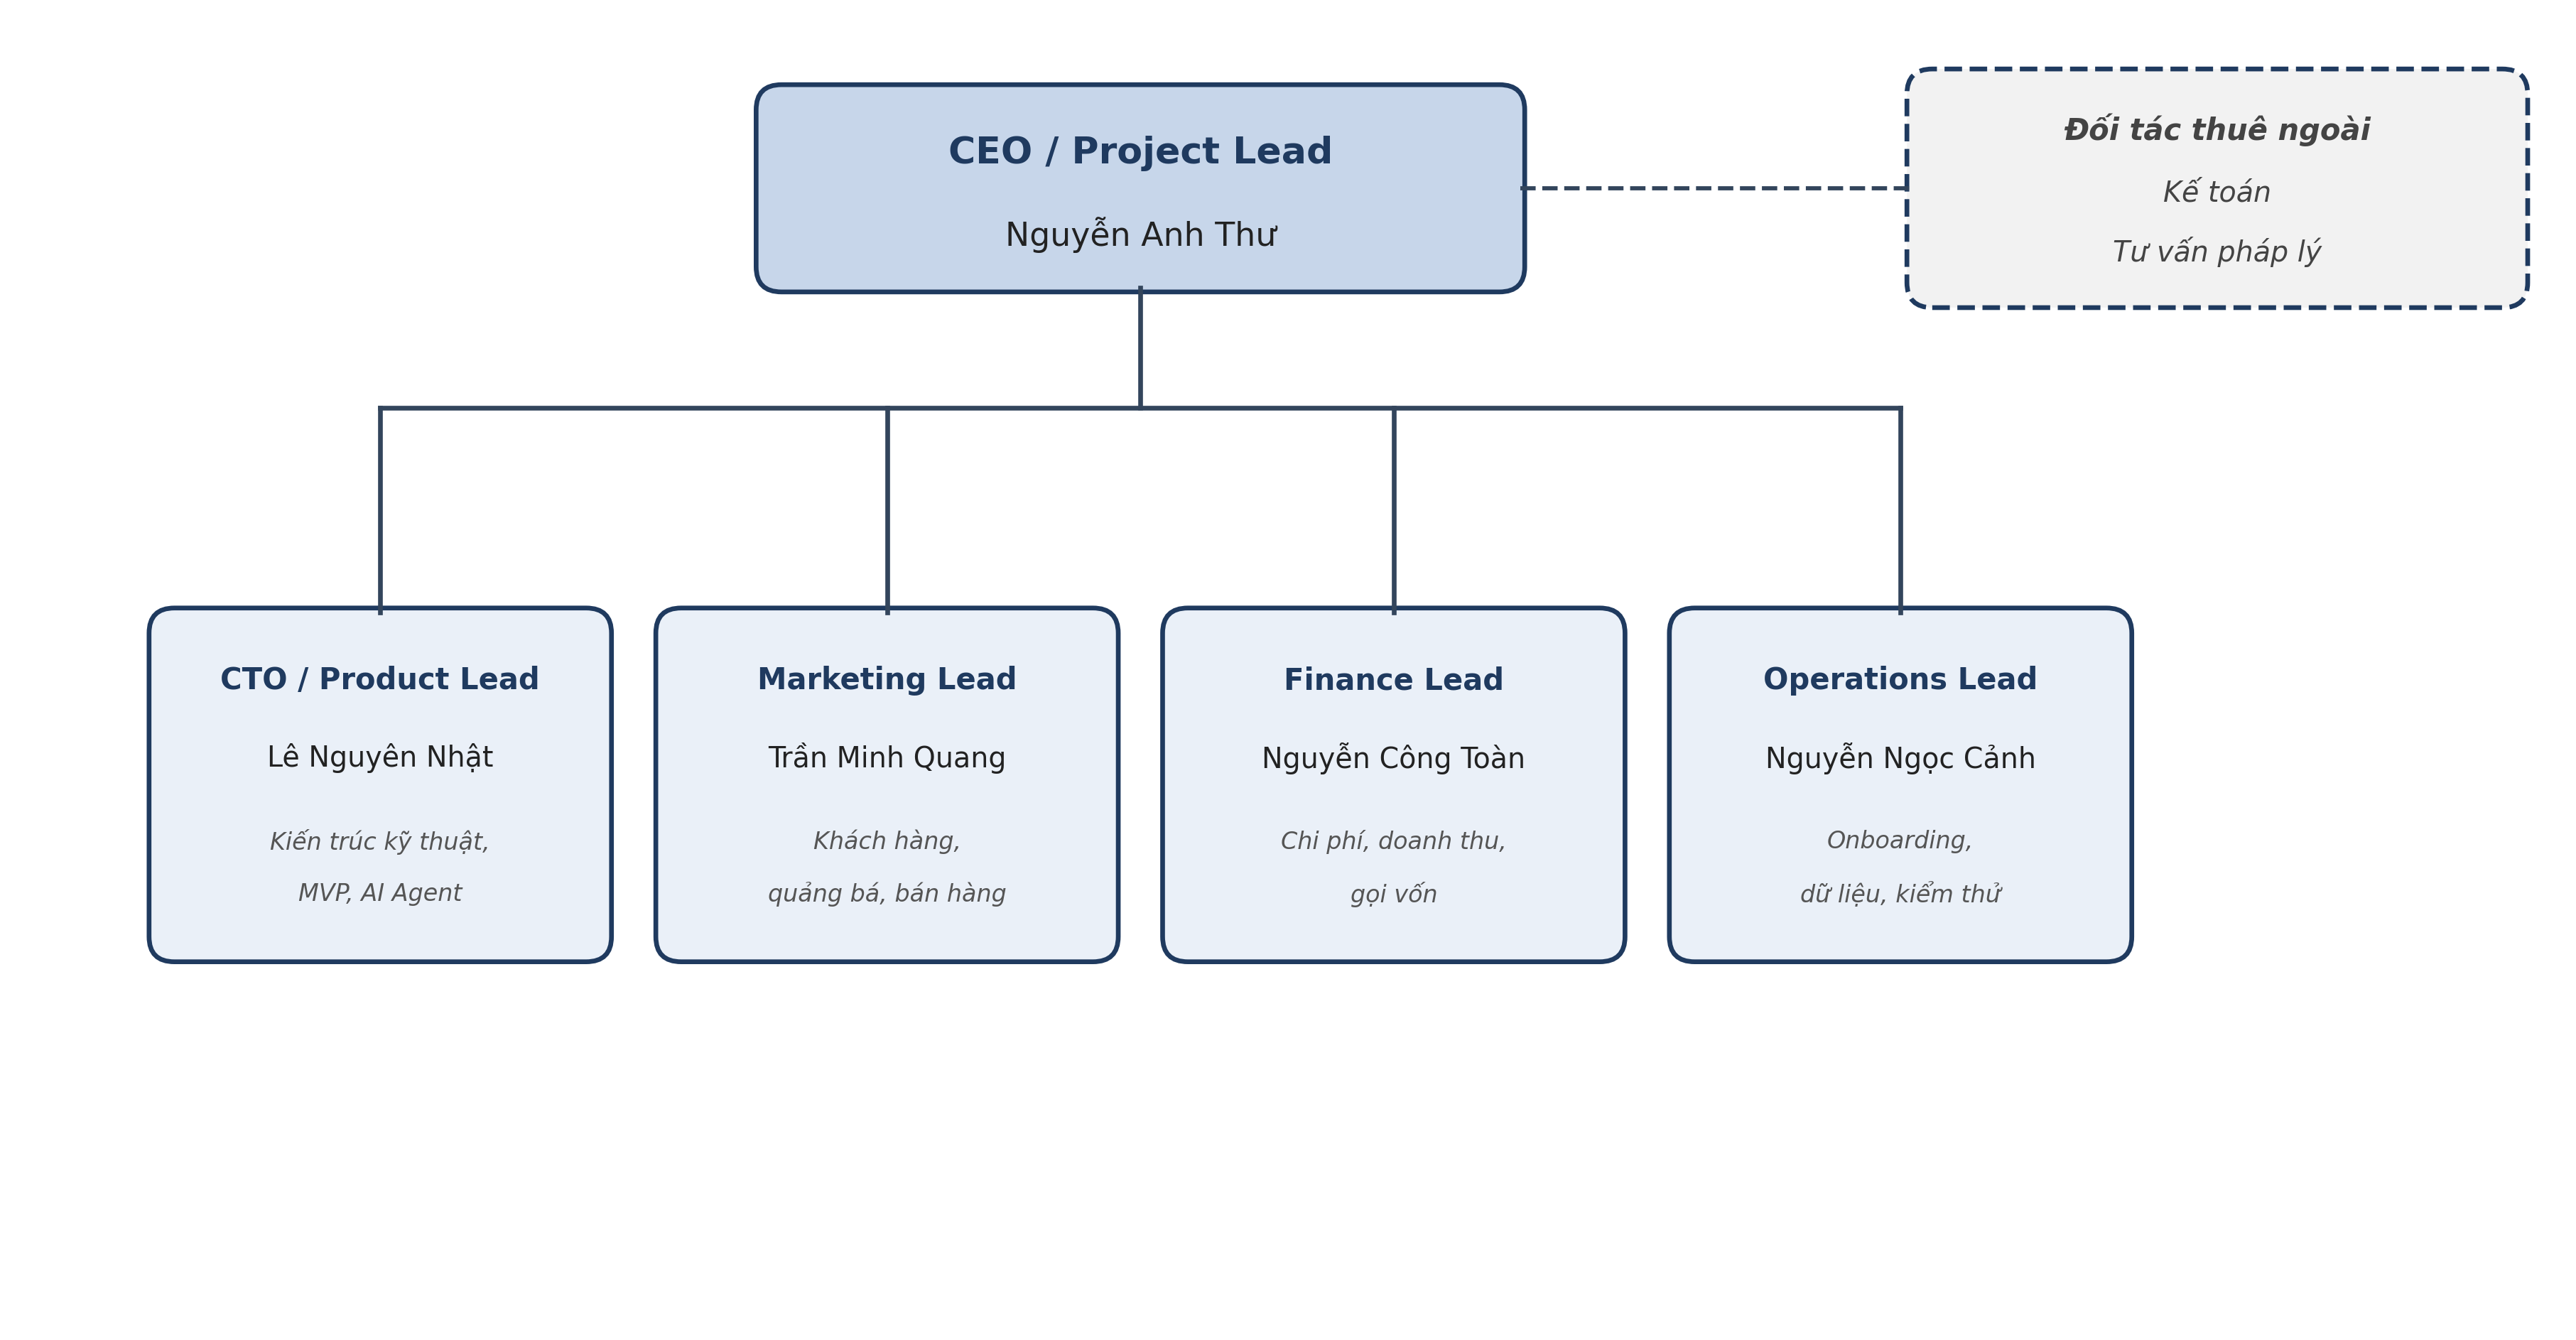
\includegraphics[width=\textwidth]{imgs/co_cau_to_chuc.png}
    \caption{Cơ cấu tổ chức nhóm/startup dự kiến trong giai đoạn đầu}
    \label{fig:cocau-to-chuc}
\end{figure}

CEO/Project Lead giữ vai trò định hướng chiến lược và điều phối chung, đồng thời
là đầu mối ra quyết định cuối cùng giữa bốn mảng chức năng. Bốn vị trí trưởng
mảng -- Công nghệ/Sản phẩm, Marketing, Tài chính và Vận hành -- chịu trách
nhiệm trọn vẹn cho lĩnh vực của mình và \textbf{phối hợp ngang} với nhau theo
từng đầu việc cụ thể: Finance Lead làm việc sát với CTO để kiểm soát chi phí
API/cloud/GPU và với Marketing Lead để thống nhất chính sách giá; Operations Lead
phối hợp với CTO về dữ liệu vận hành và với Marketing Lead về phản hồi của khách
hàng. Các nghiệp vụ kế toán, thuế và pháp lý được thể hiện bằng khối nét đứt, cho
thấy đây là quan hệ đối tác thuê ngoài thay vì vị trí nội bộ.

Nhóm ý thức rằng cơ cấu phẳng tuy phù hợp ở giai đoạn đầu nhưng sẽ tới hạn khi
quy mô mở rộng, dễ phát sinh chồng chéo trách nhiệm và nghẽn trong phối hợp nếu
không được điều chỉnh kịp thời. Vì vậy, nhóm chủ động dự kiến lộ trình tiến hóa:
khi sản phẩm được kiểm chứng và doanh nghiệp tăng trưởng, cơ cấu sẽ được chuyên
môn hóa dần thành các bộ phận rõ ràng (Công nghệ \& Sản phẩm, Tăng trưởng \&
Marketing, Tài chính \& Hành chính -- Nhân sự, Vận hành) và bổ sung dần các tầng
quản lý cùng nhân sự còn thiếu. Kế hoạch bổ sung năng lực và nhân sự theo từng
giai đoạn được trình bày chi tiết ở Mục~1.6 và Mục~1.7.